\section{Experimental Results}

\subsection{Results for different cups}

\begin{table*} 
\centering 
\begin{tabular}{l l c c c c c c} 
\toprule % Top horizontal line
 & & & \multicolumn{5}{c}{\textbf{Acceleration Approach}} \\ 
\cmidrule(l){4-7} 
\textbf{Type of Cup} &  &  & \multicolumn{2}{c}{Training Set} & \multicolumn{2}{c}{Testing Set} &\\ % Column names row
\cmidrule(l){4-7} 
\textbf{Train} & \textbf{Test} & \diagbox{Predicted}{Real} & Empty & Full & Empty & Full &\\ % Column names row
\midrule % In-table horizontal line

 & \textcolor{Yellow}{Red Cup}  & \multirow{2}{*}{Not Careful}  & \multirow{2}{*}{0.688} & \multirow{2}{*}{\textcolor{Grey}{0.15}} & \multirow{2}{*}{\textbf{0.46}} & \multirow{2}{*}{\textcolor{Grey}{0.1}} \\ %
\textcolor{Yellow}{Transparent Cup} & \textcolor{Yellow}{Champagne} & \multirow{2}{*}{ Careful} & \multirow{2}{*}{\textcolor{Grey}{0.312}} &  \multirow{2}{*}{0.85} & \multirow{2}{*}{\textcolor{Grey}{0.54}} & \multirow{2}{*}{\textbf{0.90}} \\ 
 & \textcolor{Green}{Wine Glass} & & & & & \\ % 
 
 \cmidrule(l){2-7} 
 & \textcolor{Yellow}{Transparent Cup} & & \multirow{2}{*}{0.5} & \multirow{2}{*}{\textcolor{Grey}{0.1}} & \multirow{2}{*}{\textbf{0.53}} & \multirow{2}{*}{\textcolor{Grey}{0.15}} \\ % 
\textcolor{Yellow}{Champagne} & \textcolor{Yellow}{Red Cup} & & \multirow{2}{*}{\textcolor{Grey}{0.5}} & \multirow{2}{*}{0.9} & \multirow{2}{*}{\textcolor{Grey}{0.47}} & \multirow{2}{*}{\textbf{0.85}}\\ % 
 & \textcolor{Green}{Wine Glass} &  & &  &  & \\ % 
 
 \cmidrule(l){2-7} 
 & \textcolor{Yellow}{Transparent Cup} & & \multirow{2}{*}{0.47} & \multirow{2}{*}{\textcolor{Grey}{0}} & \multirow{2}{*}{\textbf{0.5}} & \multirow{2}{*}{\textcolor{Grey}{0.16}} \\ % 
\textcolor{Yellow}{Red Cup} & \textcolor{Yellow}{Champagne} & & \multirow{2}{*}{\textcolor{Grey}{0.53}} & \multirow{2}{*}{1} & \multirow{2}{*}{\textcolor{Grey}{0.5}} & \multirow{2}{*}{\textbf{0.84}}\\ % 
 & \textcolor{Green}{Wine Glass} &  & &  &  & \\ % 
 
 \cmidrule(l){2-7} 
 & \textcolor{Yellow}{Transparent Cup} & & \multirow{2}{*}{0.5} & \multirow{2}{*}{\textcolor{Grey}{0.25}} & \multirow{2}{*}{\textbf{0.59}} & \multirow{2}{*}{\textcolor{Grey}{0.17}}\\ % 
\textcolor{Green}{Wine Glass} & \textcolor{Yellow}{Red Cup} & & \multirow{2}{*}{\textcolor{Grey}{0.5}} & \multirow{2}{*}{0.75} & \multirow{2}{*}{\textcolor{Grey}{0.41}} & \multirow{2}{*}{\textbf{0.83}}\\ % 
 & \textcolor{Yellow}{Champagne} & &  &  &  & \\ % 
 
  \cmidrule(l){2-7} 
 & \textcolor{Yellow}{Red Cup} & & \multirow{2}{*}{0.688} & \multirow{2}{*}{\textcolor{Grey}{0.15}} & \multirow{2}{*}{\textbf{0.52}} & \multirow{2}{*}{\textcolor{Grey}{0.04}} \\
\textcolor{Yellow}{Transparent Cup} & & & \multirow{2}{*}{\textcolor{Grey}{0.312}} & \multirow{2}{*}{0.85} & \multirow{2}{*}{\textcolor{Grey}{0.48}} & \multirow{2}{*}{\textbf{0.96}}\\ % 
 & \textcolor{Yellow}{Champagne} &  & &  &  &  \\ % 
 
  \cmidrule(l){2-7} 
 & \textcolor{Yellow}{Transparent Cup} & & \multirow{2}{*}{0.5} & \multirow{2}{*}{\textcolor{Grey}{0.1}} & \multirow{2}{*}{\textbf{0.55}} & \multirow{2}{*}{\textcolor{Grey}{0.08}} \\ % 
\textcolor{Yellow}{Champagne} &  & & \multirow{2}{*}{\textcolor{Grey}{0.5}} & \multirow{2}{*}{0.9} & \multirow{2}{*}{\textcolor{Grey}{0.45}} & \multirow{2}{*}{\textbf{0.92}}\\ %
 & \textcolor{Yellow}{Red Cup} & &  &  &  & \\ %   
 
  \cmidrule(l){2-7} 
 & \textcolor{Yellow}{Transparent Cup} & & \multirow{2}{*}{0.47} & \multirow{2}{*}{\textcolor{Grey}{0}} & \multirow{2}{*}{\textbf{0.5}} & \multirow{2}{*}{\textcolor{Grey}{0.09}} \\ % 
\textcolor{Yellow}{Red Cup} &  & & \multirow{2}{*}{\textcolor{Grey}{0.53}} & \multirow{2}{*}{1} & \multirow{2}{*}{\textcolor{Grey}{0.5}} &  \multirow{2}{*}{\textbf{0.91}}\\ % 
 & \textcolor{Yellow}{Champagne} &  &  &  & \\ % 
 
  \cmidrule(l){2-7} 
\textcolor{Yellow}{Transparent Cup}  &  & & \multirow{2}{*}{0.61} & \multirow{2}{*}{\textcolor{Grey}{0.15}} & \multirow{2}{*}{\textbf{0.625}} & \multirow{2}{*}{\textcolor{Grey}{0.3}} \\ % 
 & \textcolor{Yellow}{Champagne}  & & \multirow{2}{*}{\textcolor{Grey}{0.39}} & \multirow{2}{*}{0.85} & \multirow{2}{*}{\textcolor{Grey}{0.375}} &  \multirow{2}{*}{\textbf{0.7}}\\ % 
\textcolor{Yellow}{Red Cup}  & &  &  &  & \\ % 
 
\bottomrule % Bottom horizontal line
\end{tabular}
\caption{One vs Rest Classification. Training set: One cup type; Testing set: Other cup types. \textcolor{Yellow}{Plastic cups}; \textcolor{Green}{Glass cups}}
\label{tab:one_vs_all} 
\end{table*}

Conclusions from Table \ref{tab:one_vs_all}:
Training on one plastic and testing on the rest: 86\% $\pm$ 2.9\% Full cups are Careful, 49.6\% $\pm$ 2.9\% Empty cups are NOT Careful. Training on one plastic and testing on other plastics: 93\% $\pm$ 2.2\% Full cups are Careful, 52\% $\pm$ 2.1\% Empty cups are NOT Careful. Training on glass and testing on plastics: 83\% Full cups are Careful,	59\% Empty cups are NOT Careful.

Soft plastics vs Rigid plastics: 70\% vs 92\% for Full cups are Careful, 63\% vs 55\% for Empty cups are NOT Careful. 

The classifier predicts that unknown Full cups are predominantly classified as Careful manipulations irrespective of the type of cup the model is trained on.
Training and testing on plastics achieves the best results since it induces similar characteristics (e.g. risk of breaking, friction, weight, etc.) 
Training a model on glass and testing on plastics worsens the likelihood of detecting Full cups as Careful manipulations which could be induced by different characteristics being present (glass can break, and glass is heavier than plastic)
Soft plastics vs Rigid plastics: 		
Soft is difficult to handle when full of water, deformable;
Rigid plastic is closer to a glass, not deformable; 
A model trained on soft plastics learns that Full cups actions are extremely difficult, hence Full cups actions for Rigid plastics have a higher tendency to be classified NOT Careful.
A model trained on Rigid plastics learns the opposite hence Full cups actions for soft plastics are mostly classified as Careful manipulations

\subsection{Results for different datasets}

%%%%% EPFL vs EPFL (rest) dataset %%%%%%%%%%%%

\begin{table} 
\centering 
\resizebox{\columnwidth}{!}{%
\begin{tabular}{l l c c c c c c} 
\toprule % Top horizontal line
 & & & \multicolumn{5}{c}{\textbf{Acceleration Approach}} \\ 
\cmidrule(l){4-7} 
\textbf{} &  &  & \multicolumn{2}{c}{Training Set} & \multicolumn{2}{c}{Testing Set} &\\ % Column names row
\cmidrule(l){4-7} 
\textbf{Train} & \textbf{Test} & \diagbox{Predicted}{Real} & Empty & Full & Empty & Full &\\ % Column names row
\midrule % In-table horizontal line

\multirow{2}{*}{EPFL 10\%}  & \multirow{2}{*}{EPFL 90\%} & Not Careful & 0.83 & \textcolor{Grey}{0} & \textbf{0.53} &  \textcolor{Grey}{0.19}\\
  &   & Careful & \textcolor{Grey}{0.17} & 1 & \textcolor{Grey}{0.47} & \textbf{0.81} \\
  
  \cmidrule(l){2-7} 
\multirow{2}{*}{EPFL 20\%}  & \multirow{2}{*}{EPFL 80\%} &  & 0.89 & \textcolor{Grey}{0.12} & \textbf{0.5} &  \textcolor{Grey}{0.16}\\
  &   &  & \textcolor{Grey}{0.11} & 0.88 & \textcolor{Grey}{0.5} & \textbf{0.84}  \\ 
  
\cmidrule(l){2-7} 
\multirow{2}{*}{EPFL 30\%}  & \multirow{2}{*}{EPFL 70\%} &  & 0.69 & \textcolor{Grey}{0.09} & \textbf{0.51} &  \textcolor{Grey}{0.15}\\
  &   &  & \textcolor{Grey}{0.31} & 0.91 & \textcolor{Grey}{0.15} & \textbf{0.85}  \\
  
\cmidrule(l){2-7} 
\multirow{2}{*}{EPFL 40\%}  & \multirow{2}{*}{EPFL 60\%} &  & 0.6 & \textcolor{Grey}{0.13} & \textbf{0.55} &  \textcolor{Grey}{0.1}\\
  &   &  & \textcolor{Grey}{0.4} & 0.87 & \textcolor{Grey}{0.45} & \textbf{0.9}  \\

\cmidrule(l){2-7} 
\multirow{2}{*}{EPFL 50\%}  & \multirow{2}{*}{EPFL 50\%} &  & 0.61 & \textcolor{Grey}{0.16} & \textbf{0.5} &  \textcolor{Grey}{0.1}\\
  &   &  & \textcolor{Grey}{0.39} & 0.84 & \textcolor{Grey}{0.5} & \textbf{0.9}  \\
  
\cmidrule(l){2-7} 
\multirow{2}{*}{EPFL 60\%}  & \multirow{2}{*}{EPFL 40\%} &  & 0.55 & \textcolor{Grey}{0.08} & \textbf{0.5} &  \textcolor{Grey}{0.15}\\
  &   &  & \textcolor{Grey}{0.45} & 0.92 & \textcolor{Grey}{0.5} & \textbf{0.85}  \\
  
  
\midrule % In-table horizontal line
\midrule % In-table horizontal line
\end{tabular}
}
\label{tab:epfl} % A label for referencing this table elsewhere, references are used in text as \ref{label}
\caption{Training set: small size of the EPFL dataset; Testing set: the rest of the EPFL dataset.}
\end{table}

%%%%% QMUL dataset %%%%%%%%%%%%

\begin{table} 
\centering 
\resizebox{\columnwidth}{!}{%
\begin{tabular}{l l c c c c c c} 
\toprule % Top horizontal line
 & & & \multicolumn{5}{c}{\textbf{Acceleration Approach}} \\ 
\cmidrule(l){4-7} 
\textbf{} &  &  & \multicolumn{2}{c}{Training Set} & \multicolumn{2}{c}{Testing Set} &\\ % Column names row
\cmidrule(l){4-7} 
\textbf{Train} & \textbf{Test} & \diagbox{Predicted}{Real} & Empty & Full & Empty & Full &\\ % Column names row
\midrule % In-table horizontal line

\multirow{2}{*}{EPFL 10\%}  & \multirow{1}{*}{QMUL} & Not Careful & 1 & \textcolor{Grey}{0} & \textbf{0.5625} &  \textcolor{Grey}{0.2}\\
  &   & Careful & \textcolor{Grey}{0} & 1 & \textcolor{Grey}{0.4375} & \textbf{0.8} \\
  
  \cmidrule(l){2-7} 
\multirow{2}{*}{EPFL 20\%}  & \multirow{1}{*}{QMUL} &  & 0.92 & \textcolor{Grey}{0.14} & \textbf{0.5} &  \textcolor{Grey}{0.2}\\
  &   &  & \textcolor{Grey}{0.08} & 0.86 & \textcolor{Grey}{0.5} & \textbf{0.8}  \\ 
  
\cmidrule(l){2-7} 
\multirow{2}{*}{EPFL 40\%}  & \multirow{1}{*}{QMUL} &  & 0.94 & \textcolor{Grey}{0.18} & \textbf{0.5} &  \textcolor{Grey}{0.13}\\
  &   &  & \textcolor{Grey}{0.06} & 0.82 & \textcolor{Grey}{0.5} & \textbf{0.87}  \\
  
\cmidrule(l){2-7} 
\multirow{2}{*}{EPFL 50\%}  & \multirow{1}{*}{QMUL} &  & 0.7 & \textcolor{Grey}{0.29} & \textbf{0.5} &  \textcolor{Grey}{0.27}\\
  &   &  & \textcolor{Grey}{0.3} & 0.71 & \textcolor{Grey}{0.5} & \textbf{0.73}  \\
  
\midrule % In-table horizontal line
\midrule % In-table horizontal line
\end{tabular}
}
\caption{Classifier to new datasets. \\Training set: One cup type; Testing set: QMUL dataset with new people and new cup types.}
\label{tab:qmul} 
\end{table}

Conclusions on QMUL: 
For a different dataset, the classifier can continue to correctly identify manipulation of different cups: Full cup actions are predominantly classified as Careful manipulations. Even for untrained cup types and unknown people. Empty cup actions have no preference on the type of manipulation. For different data sampling rate (30 Hz instead of 120 Hz). Different acquisition technique (3D estimation from stereo vision the 3D center of mass of the object vs infra-red markers on the base of the cup)
Picking too much data will add noise to the system. It is important to not add too much data to the model has it increases the number of outliers which affect the overall representation of NOT Careful vs Careful manipulation

%%%%% IST dataset %%%%%%%%%%%%

\begin{table} 
\centering 
\resizebox{\columnwidth}{!}{%
\begin{tabular}{l l c c c c c c} 
\toprule % Top horizontal line
 & & & \multicolumn{5}{c}{\textbf{Acceleration Approach}} \\ 
\cmidrule(l){4-7} 
\textbf{} &  &  & \multicolumn{2}{c}{Training Set} & \multicolumn{2}{c}{Testing Set} &\\ % Column names row
\cmidrule(l){4-7} 
\textbf{Train} & \textbf{Test} & \diagbox{Predicted}{Real} & Empty & Full & Empty & Full &\\ % Column names row
\midrule % In-table horizontal line

\multirow{2}{*}{EPFL 10\%}  & \multirow{1}{*}{IST} & Not Careful & 0.45 & \textcolor{Grey}{0.02} & \textbf{0.65} &  \textcolor{Grey}{0.18}\\
  &   & Careful & \textcolor{Grey}{0.55} & 0.97 & \textcolor{Grey}{0.35} & \textbf{0.82} \\
  
  \cmidrule(l){2-7} 
\multirow{2}{*}{EPFL 20\%}  & \multirow{1}{*}{IST} &  & 0.58 & \textcolor{Grey}{0.11} & \textbf{0.51} &  \textcolor{Grey}{0.22}\\
  &   &  & \textcolor{Grey}{0.42} & 0.88 & \textcolor{Grey}{0.49} & \textbf{0.78}  \\ 
  
\cmidrule(l){2-7} 
\multirow{2}{*}{EPFL 40\%}  & \multirow{1}{*}{IST} &  & 0.55 & \textcolor{Grey}{0.10} & \textbf{0.52} &  \textcolor{Grey}{0.23}\\
  &   &  & \textcolor{Grey}{0.45} & 0.89 & \textcolor{Grey}{0.47} & \textbf{0.77}  \\
  
\midrule % In-table horizontal line
\midrule % In-table horizontal line
\end{tabular}
}
\caption{Classifier to new datasets. \\Training set: One cup type; Testing set: IST dataset with new people with the same cup as in the EPFL dataset}
\label{tab:ist} 
\end{table}

Conclusions on IST: 

\subsection{Discussion}

  \begin{tikzpicture}
    \draw (0,3)  node[above]{Deformable}  -- (0,-3) node[below]                 {Non-deformable}(-3,0) node[xshift=-6pt,rotate=90] {Non-breakable} -- (3,0)  node[xshift=6pt,rotate=-90] {Breakable};
    \node at (-1.5,1.5) {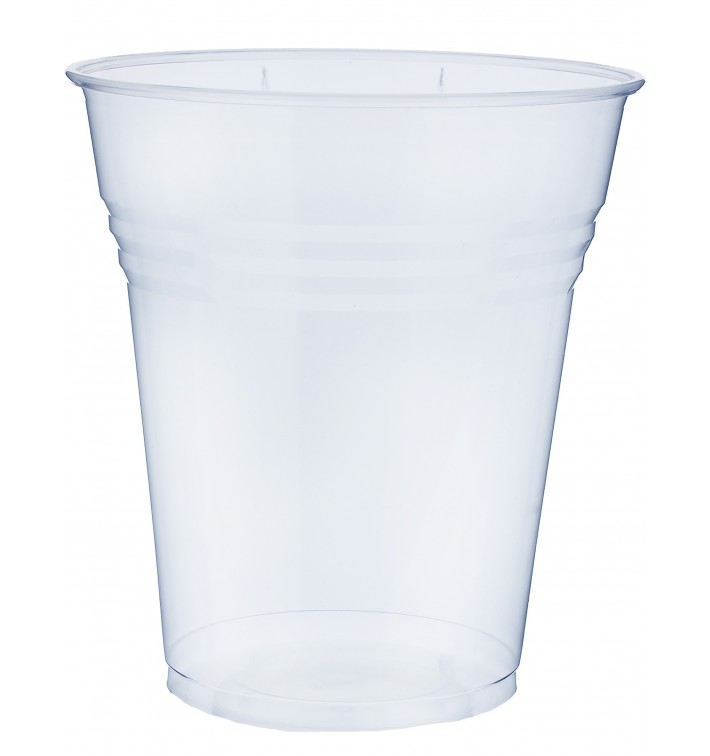
\includegraphics[width = 0.04\textwidth]{Images/transparent_cup.jpg}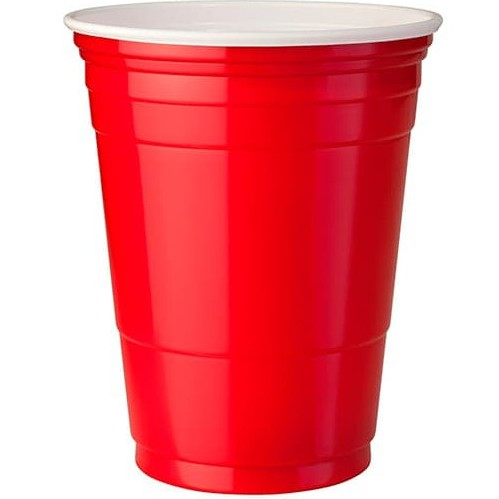
\includegraphics[width = 0.07\textwidth]{Images/red_cup.jpg}};
    \node at (1.5,1.5) {};
    \node at (-1.5,-1.5) {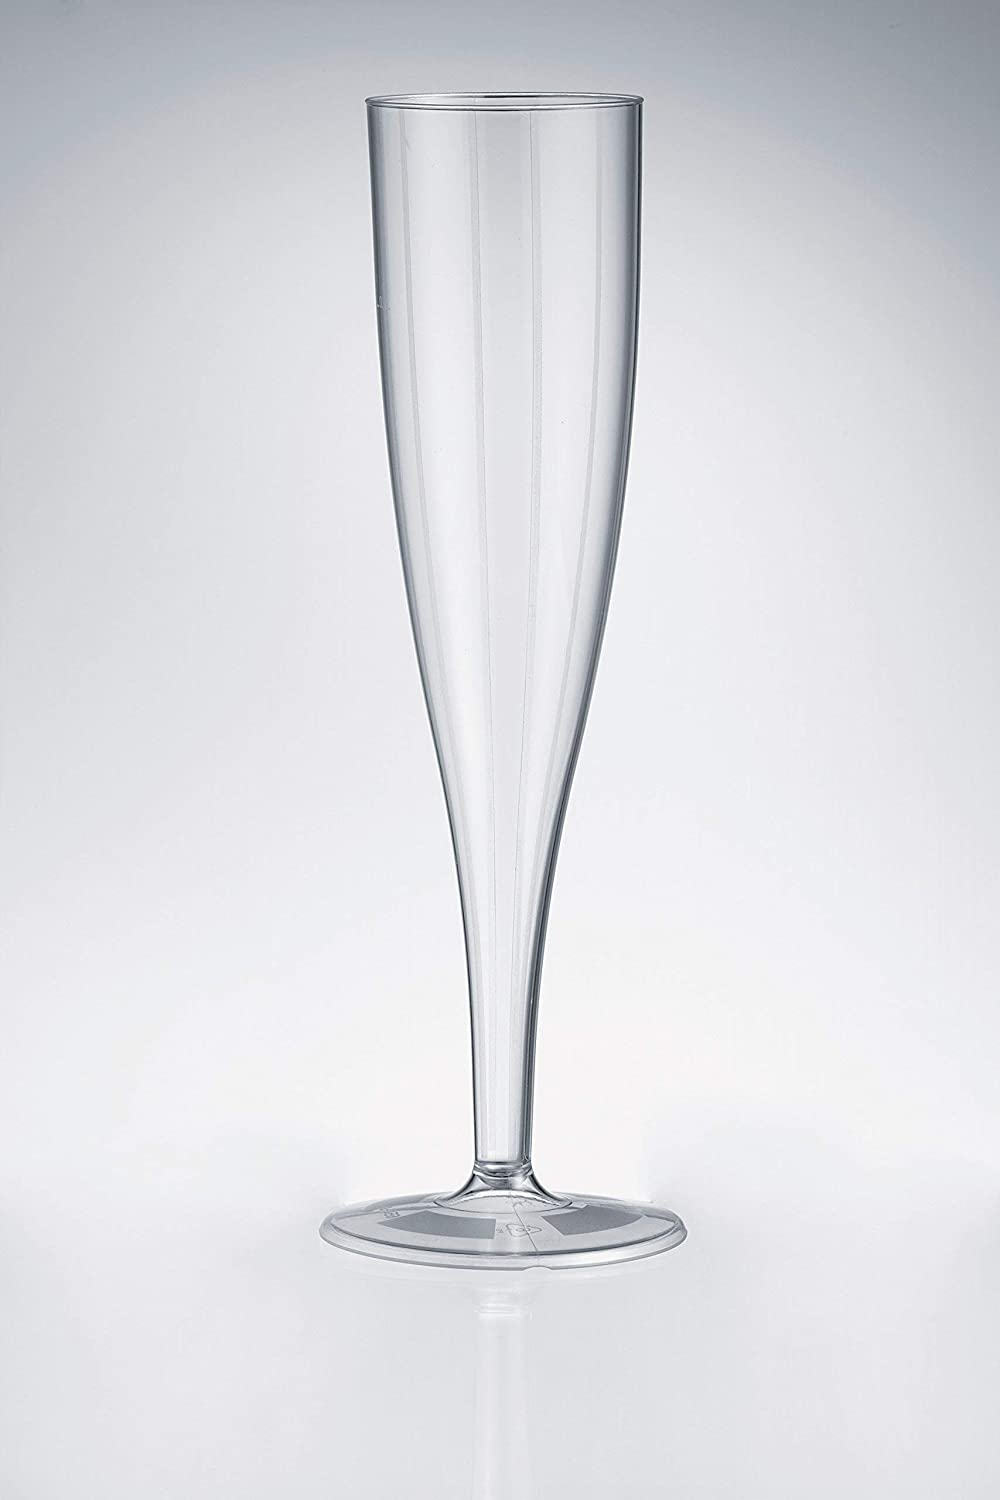
\includegraphics[width = 0.1\textwidth]{Images/champagne_cup.jpg}};
    \node at (1.5,-1.5) {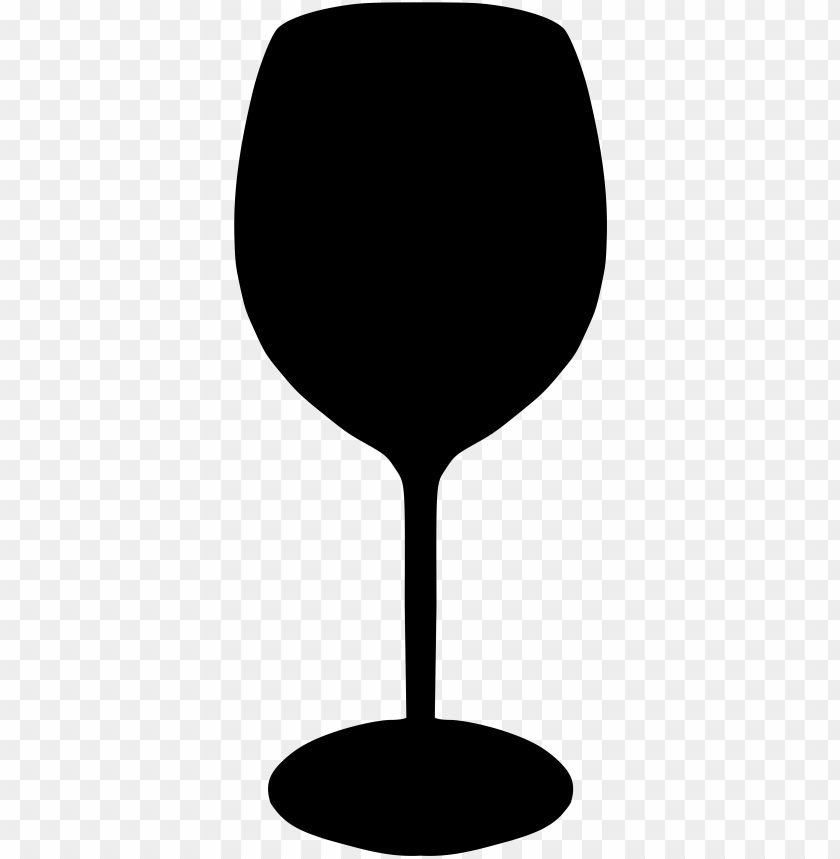
\includegraphics[width = 0.1\textwidth]{Images/wine_glass1.png}};
  \end{tikzpicture}
